% !TeX spellcheck = en_US
\documentclass[letterpaper,12pt,twoside]{report}
\usepackage{fancyhdr}
\usepackage{fullpage}
\usepackage{tikz}
\usepackage{amsmath}
\usepackage{textcomp}

\begin{document}
	\pagestyle{fancy}
	\fancyhf{}
	\fancyhead[L]{Day 29}
	\fancyhead[R]{\textit{The Calendar Project}}
	\fancyfoot[L]{Citations Involved: none}
	
	% Problem
	\paragraph{Problem}
	\begin{quote}
		\textsf{Right triangle $ABC$ has squares
			constructed on the
			legs and the
			hypotenuse. The
			vertices of the squares
			are connected to
			create hexagon
			$DEFGHI$. If $AB=3$
			cm and $BC=4$ cm,
			find the area of the hexagon.}
	\end{quote}
	
	% Graphics
	\begin{center}
		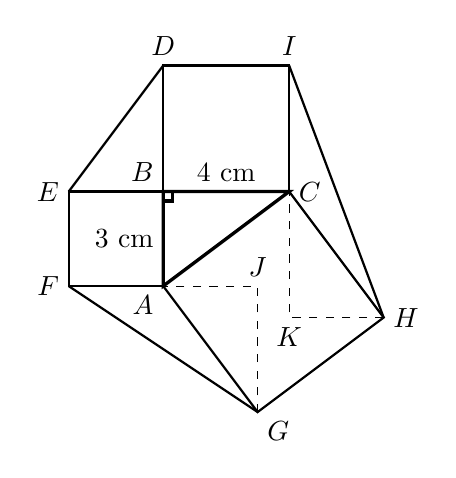
\begin{tikzpicture}[scale=0.4]
		\draw[very thick] (0,0) -- (0,-3) -- (4,0) -- cycle;
		\draw[very thick] (0,-0.3) -- (0.3,-0.3) -- (0.3,0);
		\node[above left] at (0,0) {$B$};
		\node[ right] at (4,0) {$C$};
		\node[below left] at (0,-3) {$A$};
		
		\draw[thick] (0,0) -- (0,4) -- (4,4) -- (4,0);
		\draw[thick] (0,0) -- (-3,0) -- (-3,-3) -- (0,-3);
		\draw[thick] (0,-3) -- (3,-7) -- (7,-4) -- (4,0);
		\node[above] at (0,4) {$D$};
		\node[above] at (4,4) {$I$};
		\node[left] at (-3,0) {$E$};
		\node[left] at (-3,-3) {$F$};
		\node[below right] at (3,-7) {$G$};
		\node[right] at (7,-4) {$H$};
		
		\draw[thick] (0,4) -- (-3,0);
		\draw[thick] (4,4) -- (7,-4);
		\draw[thick] (-3,-3) -- (3,-7);
		
		\node[above] at (2,0) {4 cm};
		\node[left] at (0,-1.5) {3 cm};
		
		\draw[dashed]  (3,-7) -- (3,-3) -- (0,-3);
		\draw[dashed] (7,-4) -- (4,-4) -- (4,0);
		\node[above] at (3,-3) {$J$};
		\node[below] at (4,-4) {$K$};
		
		\end{tikzpicture}
	\end{center}
	
	% Reasoning
	\paragraph{Reasoning}
	\begin{quotation}
		
		Consider the illustration above. By the Area Addition Postulate (6), $[DEFGHI]=[EDB]+[BDIC]+[CIH]+[FEBA]+[ABC]+[GACH]+[GFA]$.
		
		By the Pythagorean Theorem (5), $AB^2+BC^2=AC^2 \Rightarrow 3^2+4^2=AC^2 \Rightarrow 9+16=AC^2 \Rightarrow AC^2=25 \Rightarrow AC=\sqrt{25}=5$. Given that $BDIC$, $FEBA$, and $GACH$ are squares, and since all sides of a square are congruent by definition (4), $BD=DI=IC=CB=4$ cm, $FE=EB=BA=AF=3$ cm, and $GA=AC=CH=HG=5$ cm. Since the area formula for a square is $x^2$ where $x$ is its side length, $[BDIC]=4^2=16$, $[FEBA]=3^2=9$, and $[GACH]=5^2=25$.
		
		Draw $\overline{GJ}$ from $G$ perpendicular to $\overleftrightarrow{FA}$, and draw $\overline{HK}$ from $H$ perpendicular to $\overleftrightarrow{IC}$. As such, $\overline{GJ}$ serves as the altitude for $\triangle GFA$ by definition (3), and $\overline{HK}$ serves as the altitude for $\triangle CIH$ by definition (3). By the Angle Addition Postulate, $\text{m}\angle BAJ+\text{m}\angle JAG=\text{m}\angle BAG=\text{m}\angle BAC+\text{m}\angle CAG$ and $\text{m}\angle BCK+\text{m}\angle KCH=\text{m}\angle BCH=\text{m}\angle BCA+\text{m}\angle ACH$. Since $\angle BAF$, $\angle CAG$, $\angle ICB$, and $\angle ACH$ are internal angles of a square, they are right angles by definition (4), meaning that their measures are equal to 90\textdegree \space and that $\overline{BA}\bot\overline{AF}$, $\overline{CA}\bot\overline{AG}$, $\overline{IC}\bot\overline{CB}$, and $\overline{AC}\bot\overline{CH}$. Since $\overline{FJ}$ extends $\overline{FA}$ and $\overline{IK}$ extends $\overline{IC}$, $\angle BAJ$ and $\angle BCK$ are right angles and have a measure of 90\textdegree. After substitution, $90+\text{m}\angle JAG=\text{m}\angle BAC+90$ and $90+\text{m}\angle KCH=\text{m}\angle BCA+90$. After subtracting 90 from both sides, $\text{m}\angle JAG=\text{m}\angle BAC$ and $\text{m}\angle KCH=\text{m}\angle BCA$; therefore $\angle JAG \cong \angle BAC$ and $\angle KCH \cong \angle BCA$.
		
		$\angle AJG$ and $\angle HKC$ are right angles because it is drawn such that $\overline{GJ}\bot\overline{AJ}$ and $\overline{HK}\bot\overline{CK}$. Since all right angles are congruent, $\angle ABC \cong \angle AJG \cong \angle HKC$. Since all sides of a square are congruent by definition (4), $\overline{AG}\cong\overline{AC}\cong\overline{HC}$. By AAS congruence (1), $\triangle ABC\cong\triangle AJG\cong\triangle HKC$. $\overline{AB}\cong\overline{AJ}\cong\overline{HK}$ and $\overline{BC}\cong\overline{JG}\cong\overline{KC}$ by CPCTC (2). Thus $AB=AJ=HK=3$ and $BC=JG=KC=4$ by the definition of segment congruency and the Transitive Property.
		
	The area formula for triangles is $\frac{1}{2}bh$ where $b$ is the length of its base and $h$ is the length of its height (7). This is applied to $\triangle GFA$ and $\triangle CIH$: $[GFA]=\frac{1}{2}(AF)(JG)=\frac{1}{2}(3)(4)=6$ and $[CIH]=\frac{1}{2}(IC)(HK)=\frac{1}{2}(4)(3)=6$. Using this formula, $[EDB]=\frac{1}{2}(EB)(BD)=\frac{1}{2}(3)(4)=6$ and $[ABC]=\frac{1}{2}(BC)(AB)=\frac{1}{2}(4)(3)=6$.
	
	Recall the equation that was deducted using the Area Addition Postulate (see the first paragraph). After substitution, $[DEFGHI]=6+16+6+9+6+25+6=\boxed{74 \text{ cm}^2}$.
	
\end{quotation}
	
	\paragraph{External References}
	
	\begin{enumerate}
		\item Textbook Ch. 4, Pg. 254: Angle-Angle-Side (AAS) Congruence
		\item Textbook Ch. 4, Pg. 260: CPCTC
		\item Textbook Ch. 5, Pg. 316: Definition of triangle altitude
		\item Textbook Ch. 6, Pg. 410: Definition of a square
		\item Textbook Ch. 9, Pg. 587: Pythagorean Theorem
		\item Textbook Ch. 9, Pg. 589: Area Addition Postulate
		\item Textbook Ch. 9, Pg. 590: Area of Triangles and Trapezoids
		
	\end{enumerate}
	
\end{document}